
%----------------------------------------------------------------------------------------%
% START LaTeX preamble

% define document type, font and paper size
\documentclass[11pt,a4paper]{article}

%----------------------------------------------------------------------------------------%
% IMPORT LaTeX packages

\usepackage{inputenc}
\usepackage[ngerman, english]{babel}
\usepackage{csquotes}
\usepackage{amsmath}
\usepackage{amssymb}
\usepackage{amsfonts}
\usepackage{graphicx}
\usepackage{wrapfig}
\usepackage[margin=1.25in]{geometry}
\usepackage{pdfpages}
\usepackage{listings}
\usepackage{setspace}
\usepackage{systeme}
\usepackage{mdframed}

%----------------------------------------------------------------------------------------%
% SET user defined commands

\newcommand{\mathsym}[1]{{}}
\newcommand{\unicode}[1]{{}}

%----------------------------------------------------------------------------------------%
% IMPORT LaTeX packages to manange bibliography

% MLA, APA, or IEEE? - https://www.overleaf.com/learn/latex/Biblatex_citation_styles
\usepackage[style=apa]{biblatex}
\addbibresource{bibliography.bib}

%----------------------------------------------------------------------------------------%
% DEFINE header values

% define the cover page values
\title
{
    Computación Aplicada - Homework 04\\
    Simulation – Basics \& Integrals
}
\author
{
    Bruno González Soria          (A01169284)\\
    Antonio Osamu Katagiri Tanaka (A01212611)\\
}
\date{\today}

%----------------------------------------------------------------------------------------%
% USER-DEFINED commands

% Keywords command
\providecommand{\keywords}[1]
{
    \\
    \\
    \small
    \textbf{\textit{Keywords:}} #1
}

%----------------------------------------------------------------------------------------%

\begin{document}

%----------------------------------------------------------------------------------------%
% DEFINE listings setup

\lstset{basicstyle=\footnotesize\ttfamily,breaklines=true}
\lstset{numbers=left, numberstyle=\tiny, stepnumber=1, numbersep=10pt}

%----------------------------------------------------------------------------------------%
% CREATE the 1st page (cover page)

\maketitle

%----------------------------------------------------------------------------------------%
% DEFINE the abstract text & keywords

%\begin{abstract}
%    \emph
%    {
%        Lorem ipsum dolor sit amet, consectetur adipiscing elit, sed do eiusmod tempor incididunt ut labore et dolore magna aliqua. Ut enim ad minim veniam, quis nostrud exercitation ullamco laboris nisi ut aliquip ex ea commodo consequat. Duis aute irure dolor in reprehenderit in voluptate velit esse cillum dolore eu fugiat nulla pariatur. Excepteur sint occaecat cupidatat non proident, sunt in culpa qui officia deserunt mollit anim id est laborum.
%    }
%    \keywords{Lorem, ipsum, dolor, sit, amet}
%\end{abstract}

%----------------------------------------------------------------------------------------%
\clearpage

%----------------------------------------------------------------------------------------%
% CREATE a table of contents in a new page

\tableofcontents
\clearpage

%----------------------------------------------------------------------------------------%
% CREATE a list of figures and a list of tables in a new page

\listoffigures
%\listoftables
\lstlistoflistings
\clearpage

%----------------------------------------------------------------------------------------%
% DOCUMENT body starts here
\section{Problem I}\label{sec:p1}

\begin{figure}[!h]
\centering
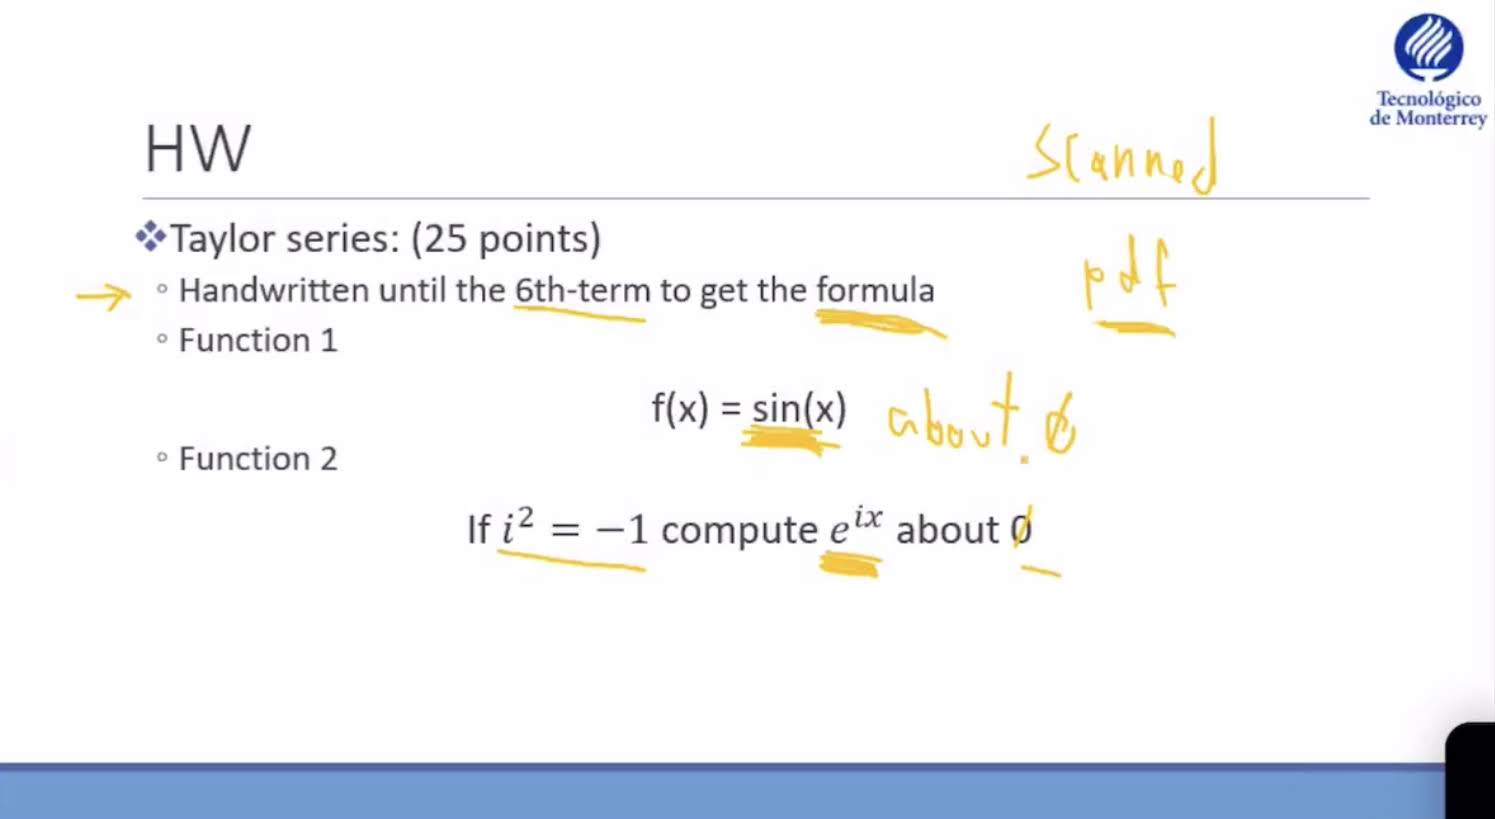
\includegraphics[width=\textwidth]{./img/instructionsP1.jpg}
\caption{Problem 1 instructions.\label{fig:P1inst}}
\end{figure}

\subsection{Function 1}\label{subsec:f1}

Figure \ref{fig:ansF1} shows the ``hadwritten" procedure to find the first six terms of the Taylor series of $ f(x) = Sin(x) $, centered at 0.

\begin{figure}[!h]
\centering
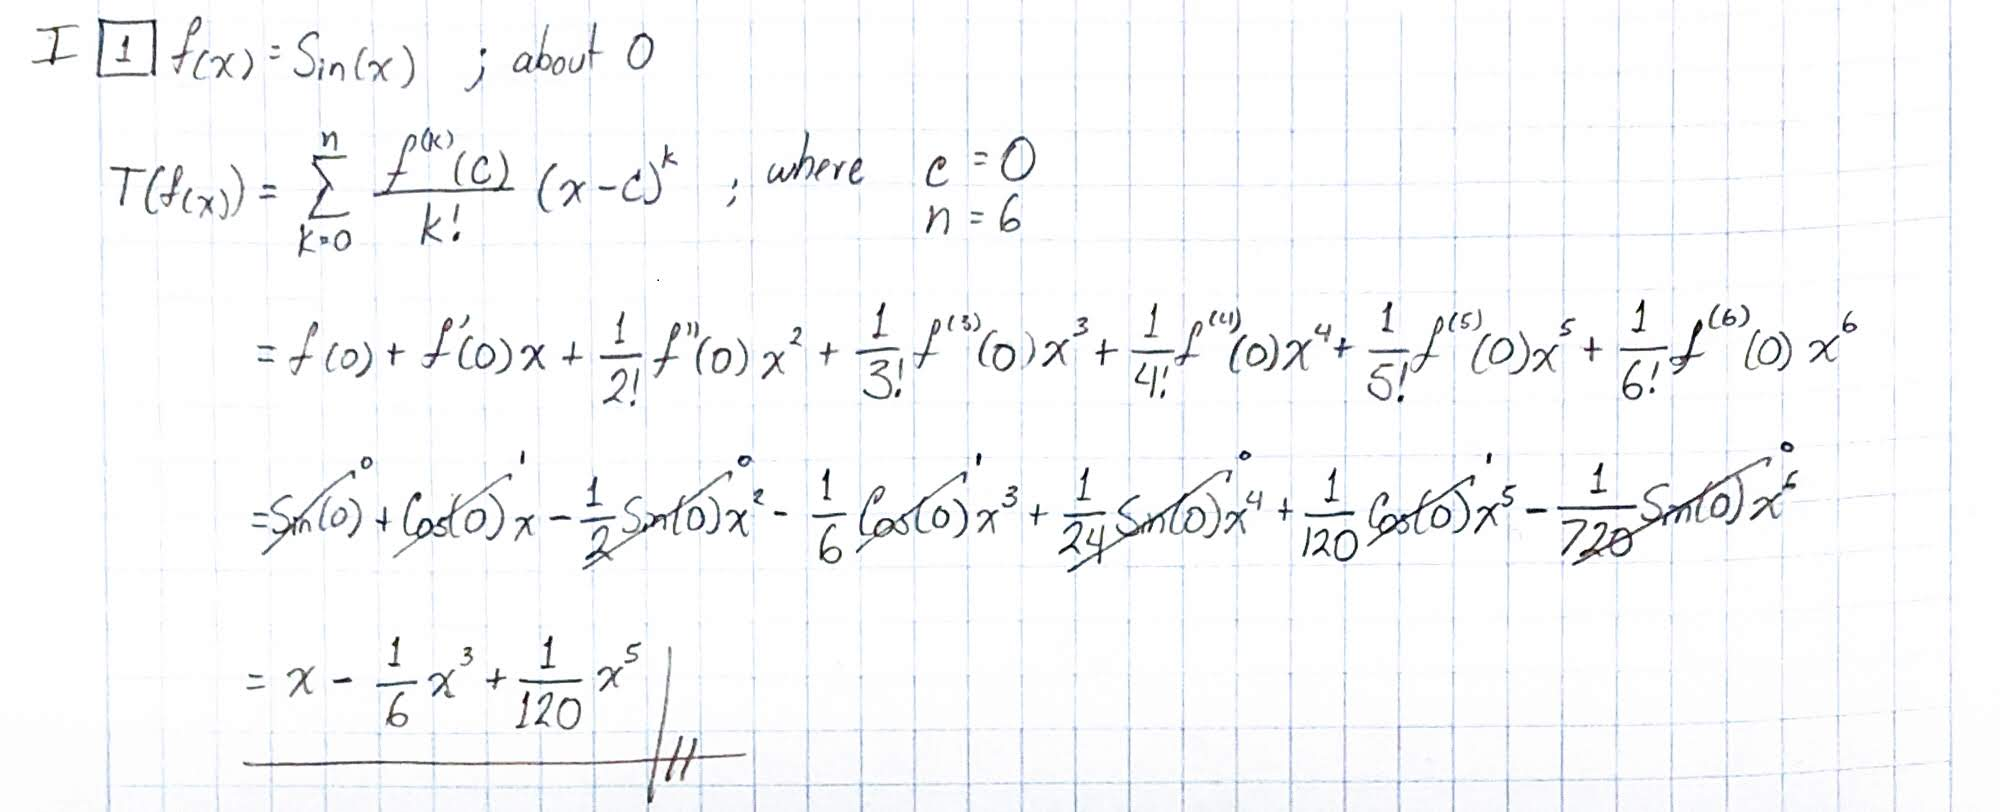
\includegraphics[width=\textwidth]{./img/P1_part1.jpg}
\caption{Taylor series until the 6th term of Function 1.\label{fig:ansF1}}
\end{figure}

\clearpage

\subsection{Function 2}\label{subsec:f2}

Figure \ref{fig:ansF2} shows the ``hadwritten" procedure to find the first six terms of the Taylor series of $ f(x) = e^{ix} $, centered at 1.

\begin{figure}[!h]
\centering
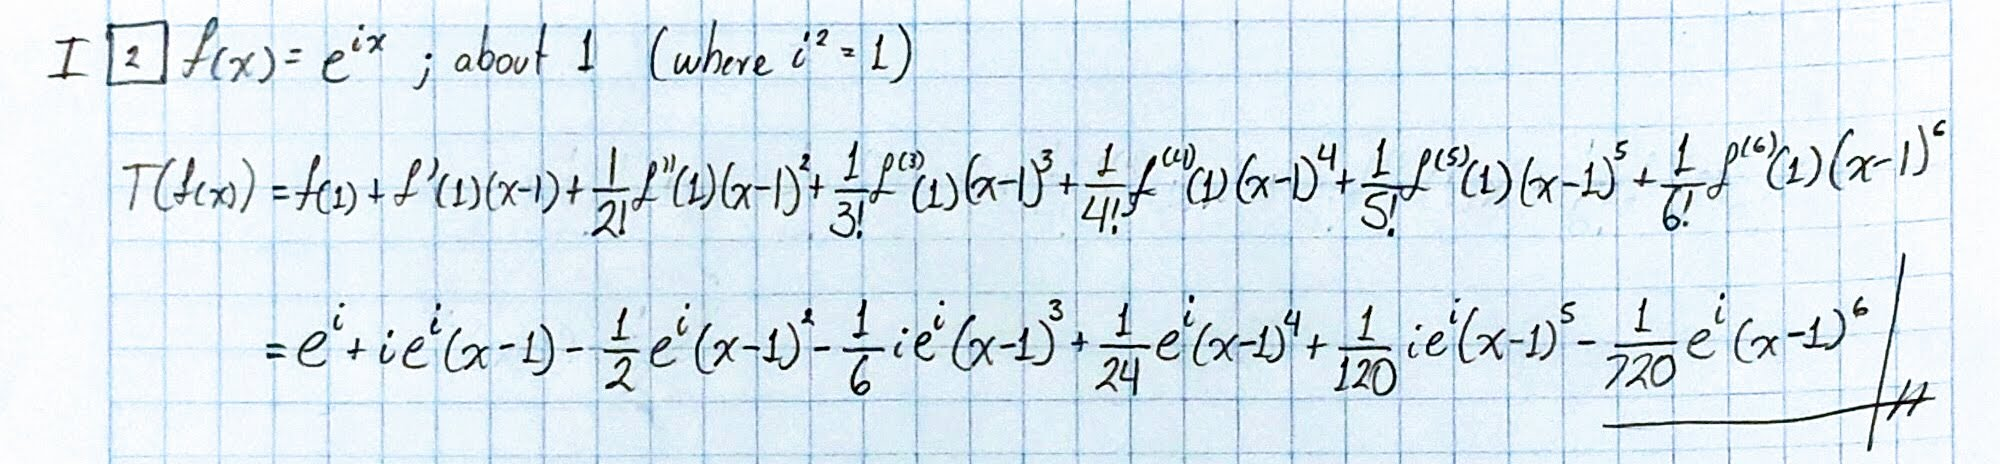
\includegraphics[width=\textwidth]{./img/P1_part2.jpg}
\caption{Taylor series until the 6th term of Function 2.\label{fig:ansF2}}
\end{figure}

\subsection{Let's plot the approximations}\label{subsec:f2}

In Listing \ref{lst:taylorPlotFunc}, function \emph{taylorPlot} is implemented to plot the Taylor approximations up to the 2nd, 4th, 6th and 8th terms. With the following properties:\\

\textbf{Parameters}:
\begin{itemize}
  \item {\textbf{f} : function\\
Vectorized function of one variable}
  \item {\textbf{c} : numeric\\
point where the series expansion will take place}
  \item {\textbf{from}, \textbf{to} : numeric\\
Interval of points to be ploted}
\end{itemize}

\textbf{Returns}:
\begin{itemize}
  \item {\textbf{void}}
\end{itemize}

\begin{lstlisting}[frame=trBL, language=R, caption="The \emph{taylorPlot} function" \label{lst:taylorPlotFunc}]
library(pracma)

taylorPlot <- function(f, c, from, to) {
  x <- seq(from, to, length.out = 100)
  yf <- f(x)
  
  yp2 <- polyval(taylor(f, c, 2), x)
  yp4 <- polyval(taylor(f, c, 4), x)
  yp6 <- polyval(taylor(f, c, 6), x)
  yp8 <- polyval(taylor(f, c, 8), x)
  
  plot(
    x,
    yf,
    xlab = "x",
    ylab = "f(x)",
    type = "l",
    main = ' Taylor Series Approximation of f(x) ',
    col = "black",
    lwd = 2
  )
  
  lines(x, yp2, col = "#c8e6c9")
  lines(x, yp4, col = "#81c784")
  lines(x, yp6, col = "#4caf50")
  lines(x, yp8, col = "#388e3c")
  
  legend(
    'topleft',
    inset = .05,
    legend = c("TS 8 terms", "TS 6 terms", "TS 4 terms", "TS 2 terms", "f(x)"),
    col = c('#388e3c', '#4caf50', '#81c784', '#c8e6c9', 'black'),
    lwd = c(1),
    bty = 'n',
    cex = .75
  )
}
\end{lstlisting}

$ f(x) = Sin(x) $ is defined as \emph{f0} and $ f(x) = e^{ix} $ is defined as \emph{f1} in  Listing \ref{lst:Functs1and2}

\begin{lstlisting}[frame=trBL, language=R, caption="Define \emph{f0} and \emph{f1}"
\label{lst:Functs1and2}]
f0 <- function(x) {
  res = sin(x)

  return(res)

}

f1 <- function(x) {
  res = exp(complex(real = 0, imaginary = 1)*x)
  
  return(res)
  
}
\end{lstlisting}

Listing \ref{lst:taylorPtFuncts1and2} shows the use of function \emph{taylorPlot} to plot the Taylor approximations of \emph{f0} and \emph{f1}. This Listing output-plots are represented within Figures \ref{fig:SinOfx_taylor} and \ref{fig:ExpOfix_taylor}

\begin{lstlisting}[frame=trBL, language=R, caption="Implement \emph{taylorPlot}"
\label{lst:taylorPtFuncts1and2}]
taylorPlot(f0, 0, -6.6, 6.6)
taylorPlot(f1, 1, -2*pi, 2*pi)
\end{lstlisting}

\begin{figure}[!h]
\centering
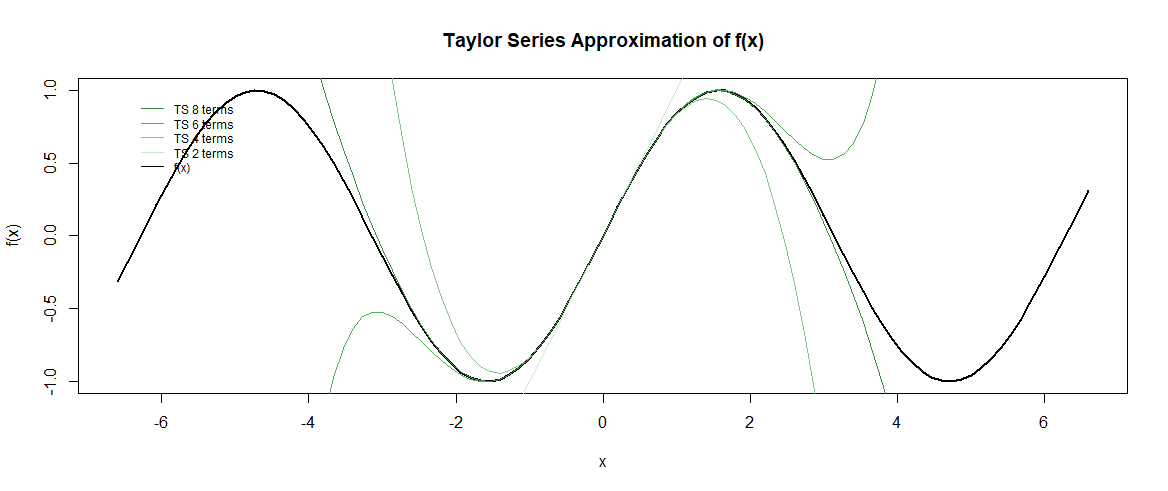
\includegraphics[width=\textwidth]{./img/SinOfx_taylor.png}
\caption{Listing \ref{lst:taylorPtFuncts1and2} output; $ f(x) = Sin(x) $ approximations, centered in 0.\label{fig:SinOfx_taylor}}
\end{figure}

\begin{figure}[!h]
\centering
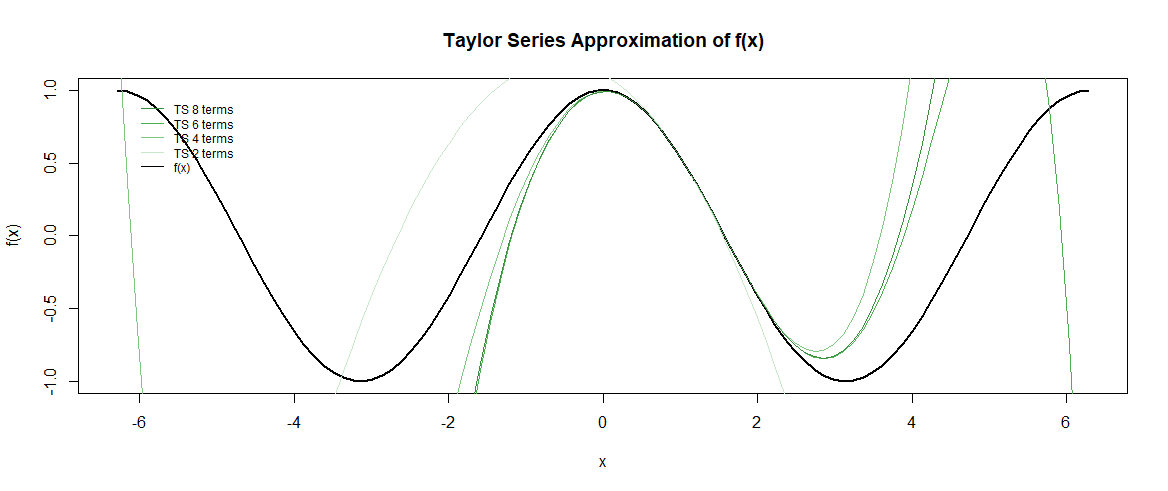
\includegraphics[width=\textwidth]{./img/ExpOfix_taylor.png}
\caption{Listing \ref{lst:taylorPtFuncts1and2} output; $ f(x) = e^{ix} $ approximations, centered in 1.\label{fig:ExpOfix_taylor}}
\end{figure}

\clearpage

%----------------------------------------------------------------------------------------%
\section{Problem II}\label{sec:p2}

\begin{figure}[!h]
\centering
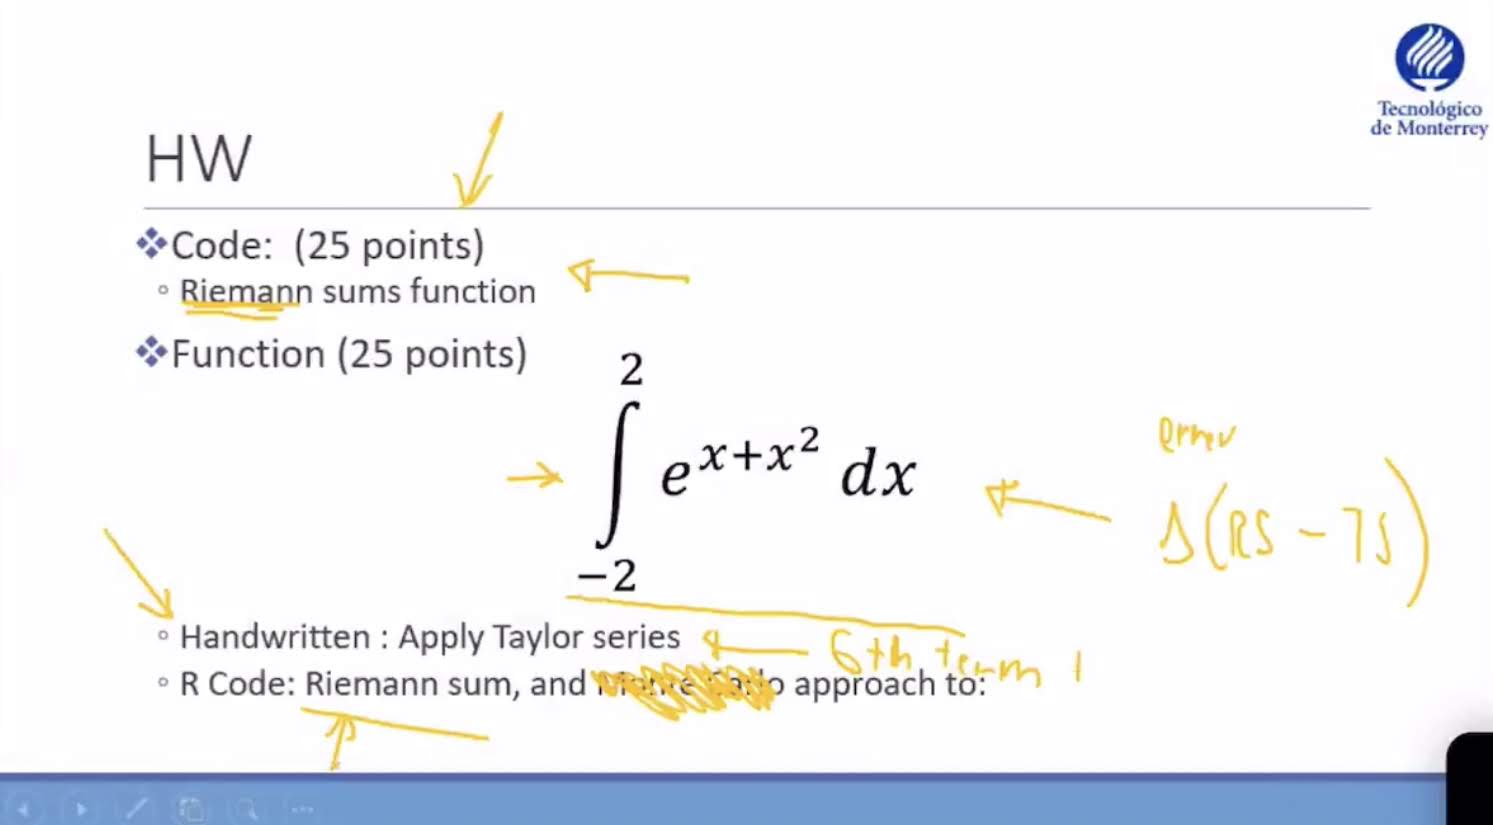
\includegraphics[width=\textwidth]{./img/instructionsP2.jpg}
\caption{Problem 2 instructions.\label{fig:P2inst}}
\end{figure}
   
In Listing \ref{lst:riemann_sumFunc}, function \emph{riemann\_sum} is implemented to compute the Riemann sum of a given function $ f(x) $ over an interval $ [a,b] $. With the following properties:\\

\textbf{Parameters}:
\begin{itemize}
  \item {\textbf{f} : function\\
Vectorized function of one variable}
  \item {\textbf{a}, \textbf{b} : numeric\\
Endpoints of the interval [a,b]}
  \item {\textbf{n} : numeric\\
Number of subintervals of equal length in the partition of [a,b]}
\end{itemize}

\textbf{Returns}:
\begin{itemize}
  \item {numeric\\
Underestimate and overestimate approximations of the integral given by the Riemann sum.}
\end{itemize}

\begin{lstlisting}[frame=trBL, language=R, caption="The \emph{Riemann} function"
\label{lst:riemann_sumFunc}]
riemann_sum <- function(f, a, b, n) {  
  # initialize values
  lower.sum <- 0
  
  upper.sum <- 0
  
  h <- (b - a) / n
  
  
  # riemann right sum
  for (i in n:1) {
    x <- a + i * h
    
    lower.sum <- lower.sum + f(x)
    
  }
  lower.sum <- h * lower.sum
  
  
  # riemann left sum
  for (i in 1:n) {
    x <- b - i * h
    
    upper.sum <- upper.sum + f(x)
    
  }
  upper.sum <- h * upper.sum
  
  
  # let's plot the curve
  integralPlot(
    f = f,
    a = a,
    b = b,
    title = expression(f(x))
  )
  
  # print/get riemann sum
  cat(sprintf(
    "The true value is between %f and %f.\n",
    as.double(lower.sum),
    as.double(upper.sum)
  ))
  
  return(c(lower.sum, upper.sum))
  
}
\end{lstlisting}

Let's solve the following integral using \emph{riemann\_sum}. Listing \ref{lst:riemannFunct4} shows the required commands.
$$ \int_{-2}^{2} e^{x+x^2} \ dx $$

\begin{lstlisting}[frame=trBL, language=R, caption="Define the function and implement \emph{riemann\_sum}"
\label{lst:riemannFunct4}]
f4 <- function(x) {
  res = exp(x + x ^ 2)
  
  return(res)
  
}

# compute riemann_sum for f4
riemann_sum(f4, -2, 2, 100000)

# let's verify our calualtion using R's function
integrate(f4, lower = -2, upper = 2)
\end{lstlisting}

\begin{lstlisting}[frame=trBL, language=R, caption="Listing \ref{lst:riemannFunct4} output"
\label{lst:riemannFunct4_out}]
> # compute riemann_sum for f4
> riemann_sum(f4, -2, 2, 100000)
The true value is between 93.170674 and 93.154833.
[1] 93.17067 93.15483

> # let's verify our calualtion using R's function
> integrate(f4, lower = -2, upper = 2)
93.16275 with absolute error < 0.00062
\end{lstlisting}

\begin{figure}[!h]
\centering
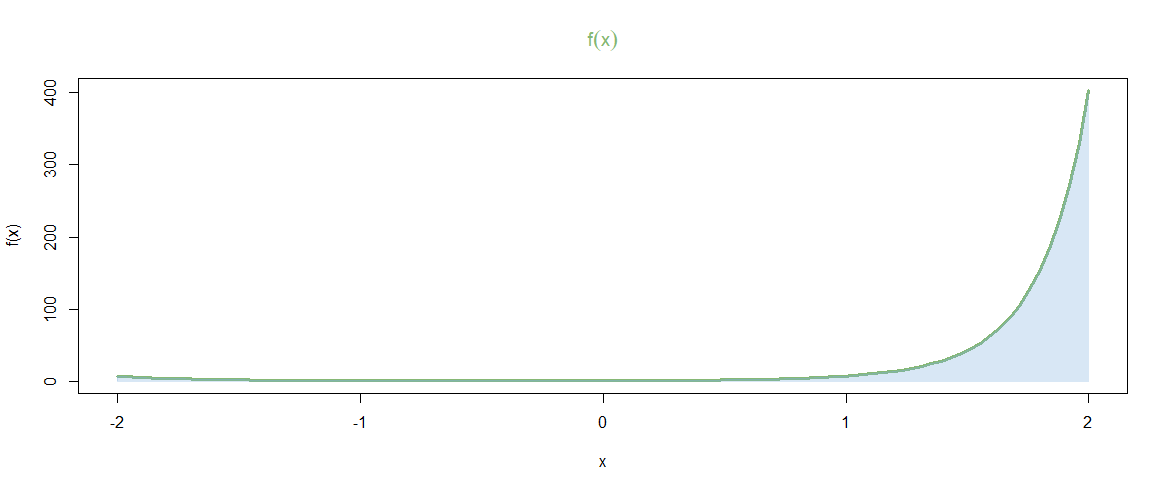
\includegraphics[width=\textwidth]{./img/ExpOfxplusxsqr.png}
\caption{Listing \ref{lst:riemannFunct4} output; $ \int_{-2}^{2} e^{x+x^2} \ dx $.\label{fig:plotArea}}
\end{figure}

* Appendix \ref{sec:appendA} implements the R function to generate plots similar to Figure \ref{fig:plotArea} \\ (, which is used within \emph{riemann\_sum}).

\clearpage

%----------------------------------------------------------------------------------------%
\section{Problem III}\label{sec:p3}

\begin{figure}[!h]
\centering
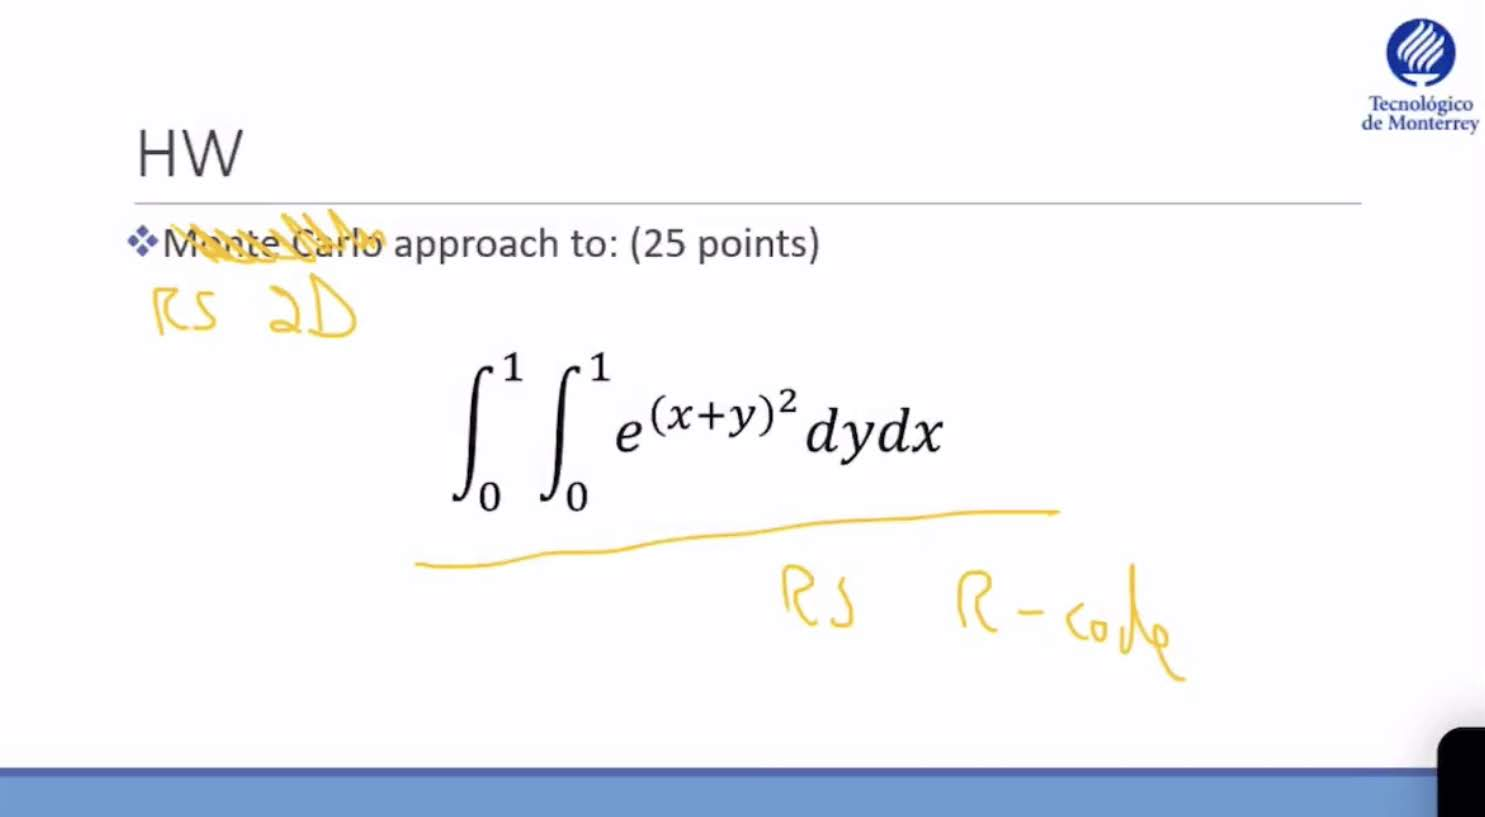
\includegraphics[width=\textwidth]{./img/instructionsP3.jpg}
\caption{Problem 3 instructions.\label{fig:P3inst}}
\end{figure}

In Listing \ref{lst:riemann2D}, function \emph{riemann\_sum\_2d} is implemented to compute the Riemann sum of a given function $ f(x,y) $ over the intervals $ [a,b] $ and $ [c,d] $. With the following properties:\\

\textbf{Parameters}:
\begin{itemize}
  \item {\textbf{f} : function\\
Vectorized function of one variable}
  \item {\textbf{a}, \textbf{b} : numeric\\
Endpoints of the interval [a,b] (inner integral)}
  \item {\textbf{c}, \textbf{d} : numeric\\
Endpoints of the interval [c,d] (outer integral)}
  \item {\textbf{nx} : numeric\\
Number of subintervals of equal length in the partition of [a,b]}
  \item {\textbf{ny} : numeric\\
Number of subintervals of equal length in the partition of [c,d]}
\end{itemize}

\textbf{Returns}:
\begin{itemize}
  \item {numeric\\
Approximations of the integral given by the Riemann 2D sum.}
\end{itemize}

\clearpage

\begin{lstlisting}[frame=trBL, language=R, caption="The \emph{Riemann 2D} function"
\label{lst:riemann2D}]
riemann_sum_2d <- function(f, a, b, c, d, nx, ny) {  
  # initialize values
  dx = (b - a) / nx
  s = 0.0
  x = a
  
  dy = (d - c) / ny
  y = c
  
  # riemann 2D sum
  for (i in 1:nx) {
    for (j in 1:ny) {
      x = a + dx / 2 + i * dx
      y = c + dy / 2 + j * dy
      f_i = f(x, y)
      s = s + f_i * dx * dy
    }
  }
  
  # print/get riemann sum
  cat(sprintf("The true value is around %f.\n",
              as.double(s)))
  
  return(s)
  
}
\end{lstlisting}

Let's solve the following integral using \emph{riemann\_sum\_2d}. Listing \ref{lst:rriemann2DFunct5} shows the required commands.
$$ \int_{0}^{1} \int_{0}^{1} e^{(x+y)^2} \ dy \ dx $$

\begin{lstlisting}[frame=trBL, language=R, caption="Define the function and implement \emph{riemann\_sum\_2d}"
\label{lst:rriemann2DFunct5}]
f5 <- function(x, y) {
  res = exp((x + y) ^ 2)
  
  return(res)
  
}

# compute riemann_sum_2d for f5
riemann_sum_2d(f5, 0, 1, 0, 1, 1000, 1000)

# let's verify our calualtion using R's function
integral2(f5, 0,1, 0,1)
\end{lstlisting}

\clearpage

\begin{lstlisting}[frame=trBL, language=R, caption="Listing \ref{lst:rriemann2DFunct5} output"
\label{lst:rriemann2DFunct5_out}]
> # compute riemann_sum_2d for f5
> riemann_sum_2d(f5, 0, 1, 0, 1, 1000, 1000)
The true value is around 4.926310.
[1] 4.92631

> # let's verify our calualtion using R's function
> integral2(f5, 0,1, 0,1)
$Q
[1] 4.899159
$error
[1] 9.974762e-16
\end{lstlisting}

\clearpage

%----------------------------------------------------------------------------------------%
\section{Problem IV}\label{sec:p4}

\begin{figure}[!h]
\centering
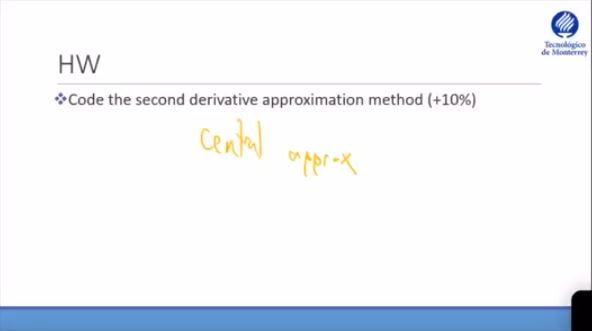
\includegraphics[width=\textwidth]{./img/instructionsP4.jpg}
\caption{Problem 4 instructions.\label{fig:P4inst}}
\end{figure}

In Listing \ref{lst:derivativeFunct}, function \emph{derivative} is implemented to compute the derivative of a function.. With the following properties:\\
  
\textbf{Parameters}:
\begin{itemize}
  \item {\textbf{f} : function $ f(x) $\\
Vectorized function of one variable}
  \item {\textbf{h} : numeric\\
Let x now change by an amount h. h is the variable that approaches 0}
\end{itemize}

\textbf{Returns}:
\begin{itemize}
  \item {function\\
Approximation of the derivative of f, given a step h.}
\end{itemize}

\clearpage

\begin{lstlisting}[frame=trBL, language=R, caption="The \emph{derivative} function"
\label{lst:derivativeFunct}]
derivative <- function(f, h) {
  return(function(x) {
    (f(x + h) - f(x)) / (h)
  })
}
\end{lstlisting}

Let's solve the following double derivative to test our function using \emph{derivative}. Listing \ref{lst:derivative} shows the required commands.
$$ \frac{d^2}{d y^2} \frac{1}{25} x^3 $$

\begin{lstlisting}[frame=trBL, language=R, caption="Define the function and implement \emph{derivative}"
\label{lst:derivative}]
f6 <- function(x) {
  res = (x^3)/25
  
  return(res)
  
}

true_d1f6 <- function(x) {
  res = (3*x^2)/25
  
  return(res)
  
}

true_d2f6 <- function(x) {
  res = (6*x)/25
  
  return(res)
  
}

# df1 = d/dx(x^4 sin(x))
#     = x^3 (4 sin(x) + x cos(x))
aprox_df1 <- derivative(f6, 0.01)

# df2 = d/dx(x^3 (4 sin(x) + x cos(x)))
#     = x^2 (8 x cos(x) - (x^2 - 12) sin(x))
aprox_df2 <- derivative(aprox_df1, 0.01)

# Let's evaluate x=pi in the second derivative df2
aprox_df2(pi)

# Let's use the eval() funtion to verify our solution. The value should be around df2(pi)
true_d2f6(pi)

# Let's plot the real and the aproximated derivatives (just to compare)
derivativePlot(f6,aprox_df1,aprox_df2,true_d1f6,true_d2f6,-0.75,0.75)
\end{lstlisting}

\clearpage

\begin{lstlisting}[frame=trBL, language=R, caption="Listing \ref{lst:derivative} output"
\label{lst:derivative_out}]
> # Let's evaluate x=pi in the second derivative df2
> aprox_df2(pi)
[1] 0.7563822
> 
> # Let's use the eval() funtion to verify our solution. The value should be around df2(pi)
> true_d2f6(pi)
[1] 0.7539822
\end{lstlisting}

Figure \ref{fig:plotderivs} shows the error between the true and approximate functions of the first and second derivatives of $ f(x) $.

\begin{figure}[!h]
\centering
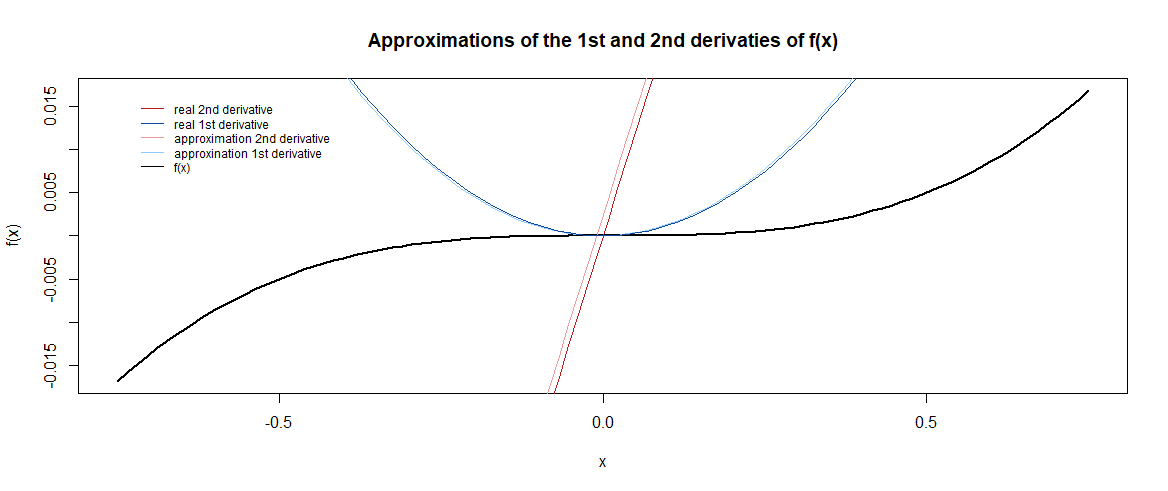
\includegraphics[width=\textwidth]{./img/1and2_derivatives.png}
\caption{Listing \ref{lst:derivative} output.\label{fig:plotderivs}}
\end{figure}

* Appendix \ref{sec:appendB} implements the R function to generate plots similar to Figure \ref{fig:plotderivs}.

%----------------------------------------------------------------------------------------%
% PRINT bibliography/references in a new page

\clearpage
\printbibliography

%----------------------------------------------------------------------------------------%
% ADD appendixes
\appendix % headings numbered with letters

\clearpage

%----------------------------------------------------------------------------------------%
\section{\emph{integralPlot} function}\label{sec:appendA}

\begin{lstlisting}[frame=trBL, language=R]
# Plotting the Areas under Curves ######################################
integralPlot <- function(f,
                         a,
                         b,
                         from = a,
                         to = b,
                         title = NULL) {
  # Plot the area under a function over the interval [a,b] between [from,to].
  #
  # Parameters
  # ----------
  # f : function
  # funtion to be ploted
  # a , b : numeric
  # Endpoints of the integral interval [a, b]
  # from , to : numeric (optional)
  # Endpoints of the plot in the x-axis [x min, x max]
  # title : expression
  # title of the plot
  #
  # Returns
  # -------
  # void
  
  x <- seq(from, to, length.out = 100) # input continuum
  y <- f(x) # output
  
  # plot the curve
  plot(
    x,
    y,
    xlim = c(from, to),
    ylim = c(ifelse(min(y) < 0, min(y), 0), max(y)),
    xlab = "x",
    ylab = "f(x)",
    main = title,
    col.main = "#86B875",
    type = "l",
    lwd = 3,
    col = "#86B875"
  )
  
  # area under the curve
  x <- seq(a, b, length.out = 100)
  y <- f(x)
  polygon(
    c(x, b, a, a),
    c(y, 0, 0, f(a)),
    border = adjustcolor("#7DB0DD", alpha.f = 0.3),
    col = adjustcolor("#7DB0DD", alpha.f = 0.3)
  )
}
\end{lstlisting}

\clearpage

%----------------------------------------------------------------------------------------%
\section{\emph{derivativePlot} function}\label{sec:appendB}

\begin{lstlisting}[frame=trBL, language=R]
# Plotting the 1ST and 2ND DERIVATIVES ################################
library(pracma)

derivativePlot <- function(f,
                           ap_df1, ap_df2,
                           tr_df1, tr_df2,
                           from, to) {
  # Plot the f and its 1st and 2nd derivatives between [from,to].
  #
  # Parameters
  # ----------
  # f : function
  # funtion to be ploted
  # ap_df1 , ap_df2 : function
  # aproximation of the 1st and 2nd derivatives of f (Normally, these are
  # generated by the derivative function)
  # tr_df1 , tr_df2 : function
  # functions that represent the true 1st and 2nd derivatives of f
  # from , to : numeric
  # Endpoints of the plot in the x-axis [x min, x max]
  #
  # Returns
  # -------
  # void
  
  x <- seq(from, to, length.out = 100)
  
  yf <- f(x)
  ap_yp2 <- ap_df1(x)
  ap_yp4 <- ap_df2(x)
  tr_yp6 <- tr_df1(x)
  tr_yp8 <- tr_df2(x)
  
  plot(
    x, yf,
    xlab = "x",
    ylab = "f(x)",
    type = "l",
    main = ' Approximations of the 1st and 2nd derivatives of f(x) ',
    col = "black",
    lwd = 2
  )
  
  lines(x, ap_yp2, col = "#90caf9") # blue lighten-3
  lines(x, ap_yp4, col = "#ef9a9a") # red lighten-3
  lines(x, tr_yp6, col = "#0d47a1") # blue darken-4
  lines(x, tr_yp8, col = "#b71c1c") # red darken-4
  
  legend(
    'topleft', inset = .05,
    legend = c("real 2nd derivative", "real 1st derivative", "approximation 2nd derivative", "approxination 1st derivative", "f(x)"),
    col = c('#b71c1c', '#0d47a1', '#ef9a9a', '#90caf9', 'black'),
    lwd = c(1), bty = 'n', cex = .75
  )
}
\end{lstlisting}

\clearpage

%----------------------------------------------------------------------------------------%
\section{Full R Script}\label{sec:fullScript}

\begin{lstlisting}[frame=trBL, language=R]
#**********************************************************************
#* AUTHOR(S) :
#*     Bruno Gonzalez Soria          (A01169284)
#*     Antonio Osamu Katagiri Tanaka (A01212611)
#*
#* FILENAME :
#*     Homework4.R
#*
#* DESCRIPTION :
#*     Simulations (Ene 19 Gpo 1)
#*     Homework 4
#*
#* NOTES :
#*     - https://www.math.ubc.ca/~pwalls/math-python/integration/riemann-sums/
#*     - https://activecalculus.org/multi/S-11-1-Double-Integrals-Rectangles.html
#*     - http://math.colgate.edu/faculty/valente/math113/supplements/section151handout.pdf
#*     - http://hplgit.github.io/Programming-for-Computations/pub/p4c/p4c-sphinx-Python/._pylight004.html
#*     - https://rstudio-pubs-static.s3.amazonaws.com/131664_1858eec97df54c9b8d5edcd8b22e5818.html
#*
#* START DATE :
#*     21 Feb 2019
#**********************************************************************

# Install required libraries
#install.packages('pracma', dependencies=TRUE);

# Plotting the Areas under Curves #####################################
integralPlot <- function(f,
                         a,
                         b,
                         from = a,
                         to = b,
                         title = NULL) {
  # Plot the area under a function over the interval [a,b] between [from,to].
  #
  # Parameters
  # ----------
  # f : function
  # funtion to be ploted
  # a , b : numeric
  # Endpoints of the integral interval [a, b]
  # from , to : numeric (optional)
  # Endpoints of the plot in the x-axis [x min, x max]
  # title : expression
  # title of the plot
  #
  # Returns
  # -------
  # void
  
  x <- seq(from, to, length.out = 100) # input continuum
  y <- f(x) # output
  
  # plot the curve
  plot(
    x,
    y,
    xlim = c(from, to),
    ylim = c(ifelse(min(y) < 0, min(y), 0), max(y)),
    xlab = "x",
    ylab = "f(x)",
    main = title,
    col.main = "#86B875",
    type = "l",
    lwd = 3,
    col = "#86B875"
  )
  
  # area under the curve
  x <- seq(a, b, length.out = 100)
  y <- f(x)
  polygon(
    c(x, b, a, a),
    c(y, 0, 0, f(a)),
    border = adjustcolor("#7DB0DD", alpha.f = 0.3),
    col = adjustcolor("#7DB0DD", alpha.f = 0.3)
  )
}

# Plotting the 1ST and 2ND DERIVATIVES ################################
library(pracma)

derivativePlot <- function(f,
                           ap_df1,
                           ap_df2,
                           tr_df1,
                           tr_df2,
                           from,
                           to) {
  # Plot the f and its 1st and 2nd derivatives between [from,to].
  #
  # Parameters
  # ----------
  # f : function
  # funtion to be ploted
  # ap_df1 , ap_df2 : function
  # aproximation of the 1st and 2nd derivatives of f (Normally, these
  # are generated by the derivative function)
  # tr_df1 , tr_df2 : function
  # functions that represent the true 1st and 2nd derivatives of f
  # from , to : numeric
  # Endpoints of the plot in the x-axis [x min, x max]
  #
  # Returns
  # -------
  # void
  
  x <- seq(from, to, length.out = 100)
  
  yf <- f(x)
  ap_yp2 <- ap_df1(x)
  ap_yp4 <- ap_df2(x)
  tr_yp6 <- tr_df1(x)
  tr_yp8 <- tr_df2(x)
  
  plot(
    x,
    yf,
    xlab = "x",
    ylab = "f(x)",
    type = "l",
    main = ' Approximations of the 1st and 2nd derivatives of f(x) ',
    col = "black",
    lwd = 2
  )
  
  lines(x, ap_yp2, col = "#90caf9") # blue lighten-3
  lines(x, ap_yp4, col = "#ef9a9a") # red lighten-3
  lines(x, tr_yp6, col = "#0d47a1") # blue darken-4
  lines(x, tr_yp8, col = "#b71c1c") # red darken-4
  
  legend(
    'topleft',
    inset = .05,
    legend = c("real 2nd derivative", "real 1st derivative", "approximation 2nd derivative", "approxination 1st derivative", "f(x)"),
    col = c('#b71c1c', '#0d47a1', '#ef9a9a', '#90caf9', 'black'),
    lwd = c(1),
    bty = 'n',
    cex = .75
  )
}

#######################################################################
# PART 1 ##############################################################
# TAYLOR SERIES

library(pracma)

taylorPlot <- function(f, c, from, to) {
  # Plot the Taylor approximations up to the 2nd, 4th, 6th and 8th terms
  #
  # Parameters
  # ----------
  # f : function
  # Vectorized function of one variable
  # c : numeric
  # point where the series expansion will take place
  # from, to : numeric
  # Interval of points to be ploted
  #
  # Returns
  # -------
  # void
  
  x <- seq(from, to, length.out = 100)
  yf <- f(x)
  
  yp2 <- polyval(taylor(f, c, 2), x)
  yp4 <- polyval(taylor(f, c, 4), x)
  yp6 <- polyval(taylor(f, c, 6), x)
  yp8 <- polyval(taylor(f, c, 8), x)
  
  plot(
    x,
    yf,
    xlab = "x",
    ylab = "f(x)",
    type = "l",
    main = ' Taylor Series Approximation of f(x) ',
    col = "black",
    lwd = 2
  )
  
  lines(x, yp2, col = "#c8e6c9")
  lines(x, yp4, col = "#81c784")
  lines(x, yp6, col = "#4caf50")
  lines(x, yp8, col = "#388e3c")
  
  legend(
    'topleft',
    inset = .05,
    legend = c("TS 8 terms", "TS 6 terms", "TS 4 terms", "TS 2 terms", "f(x)"),
    col = c('#388e3c', '#4caf50', '#81c784', '#c8e6c9', 'black'),
    lwd = c(1),
    bty = 'n',
    cex = .75
  )
}

# -----

f0 <- function(x) {
  res = sin(x)

  return(res)

}

f1 <- function(x) {
  res = exp(complex(real = 0, imaginary = 1)*x)
  
  return(res)
  
}

# -----

taylorPlot(f0, 0, -6.6, 6.6)
taylorPlot(f1, 1, -2*pi, 2*pi)


#######################################################################
# PART 2 ##############################################################
# RIEMANN SUMS FUNCTION

riemann_sum <- function(f, a, b, n) {
  # Compute the Riemann sum of f(x) over the interval [a,b].
  #
  # Parameters
  # ----------
  # f : function
  # Vectorized function of one variable
  # a , b : numeric
  # Endpoints of the interval [a,b]
  # n : numeric
  # Number of subintervals of equal length in the partition of [a,b]
  #
  # Returns
  # -------
  # numeric
  # Underestimate and overestimate approximations of the integral given by the
  # Riemann sum.
  
  # initialize values
  lower.sum <- 0
  
  upper.sum <- 0
  
  h <- (b - a) / n
  
  
  # riemann right sum
  for (i in n:1) {
    x <- a + i * h
    
    lower.sum <- lower.sum + f(x)
    
  }
  lower.sum <- h * lower.sum
  
  
  # riemann left sum
  for (i in 1:n) {
    x <- b - i * h
    
    upper.sum <- upper.sum + f(x)
    
  }
  upper.sum <- h * upper.sum
  
  
  # let's plot the curve
  integralPlot(
    f = f,
    a = a,
    b = b,
    title = expression(f(x))
  )
  
  # print/get riemann sum
  cat(sprintf(
    "The true value is between %f and %f.\n",
    as.double(lower.sum),
    as.double(upper.sum)
  ))
  
  return(c(lower.sum, upper.sum))
  
}

# -----

# let's generate some functions to test our algorithm
f2 <- function(x) {
  res = x
  
  return(res)
  
}

f3 <- function(x) {
  res = 4 / (1 + x ^ 2)
  
  return(res)
  
}

# -----

riemann_sum(f0, 0, pi / 2, 10)
riemann_sum(f2, 0, 1, 10000) # should be 0.5
riemann_sum(f3, 0, 1, 10000) # should be PI


#######################################################################
# PART 3 ##############################################################
# Integrate the function f(x)=exp(x+x^2) from -2 to 2, using Rieman sums.
f4 <- function(x) {
  res = exp(x + x ^ 2)
  
  return(res)
  
}

# plot Taylor approximations
taylorPlot(f4, 0, -2.3, 1.3)

# compute riemann_sum for f4
riemann_sum(f4, -2, 2, 100000)
# let's verify our calualtion using R's function
integrate(f4, lower = -2, upper = 2)


#######################################################################
# PART 4 ##############################################################
# RIEMANN SUMS 2D FUNCTION

riemann_sum_2d <- function(f, a, b, c, d, nx, ny) {
  # Compute the Riemann sum of f(x,y) over the intervals [a,b] and [c,d].
  #
  # Parameters
  # ----------
  # f : function
  # Vectorized function of one variable
  # a , b : numeric
  # Endpoints of the interval [a,b] (inner integral)
  # c , d : numeric
  # Endpoints of the interval [c,d] (outer integral)
  # nx : numeric
  # Number of subintervals of equal length in the partition of [a,b]
  # ny : numeric
  # Number of subintervals of equal length in the partition of [c,d]
  #
  # Returns
  # -------
  # numeric
  # Approximations of the integral given by the Riemann 2D sum.
  
  # initialize values
  dx = (b - a) / nx
  s = 0.0
  x = a
  
  dy = (d - c) / ny
  y = c
  
  # riemann 2D sum
  for (i in 1:nx) {
    for (j in 1:ny) {
      x = a + dx / 2 + i * dx
      y = c + dy / 2 + j * dy
      f_i = f(x, y)
      s = s + f_i * dx * dy
    }
  }
  
  # print/get riemann sum
  cat(sprintf("The true value is around %f.\n",
              as.double(s)))
  
  return(s)
  
}

# -----

f5 <- function(x, y) {
  res = exp((x + y) ^ 2)
  
  return(res)
  
}

# -----

# compute riemann_sum_2d for f5
riemann_sum_2d(f5, 0, 1, 0, 1, 1000, 1000)
# let's verify our calualtion using R's function
integral2(f5, 0,1, 0,1)


#######################################################################
# PART 5 ##############################################################
# 2ND DERIVATIVE APPROXIMATION

derivative <- function(f, h) {
  # Compute the derivative of a function.
  #
  # Parameters
  # ----------
  # f : function f(x)
  # Vectorized function of one variable
  # h : numeric
  # Let x now change by an amount h. h is the variable that approaches 0
  # 
  # Returns
  # -------
  # function
  # Approximations of the derivative of f, given a step h.
  
  return(function(x) {
    (f(x + h) - f(x)) / (h)
  })
}

f6 <- function(x) {
  res = (x^3)/25
  
  return(res)
  
}

true_d1f6 <- function(x) {
  res = (3*x^2)/25
  
  return(res)
  
}

true_d2f6 <- function(x) {
  res = (6*x)/25
  
  return(res)
  
}

# df1 = d/dx(x^4 sin(x))
#     = x^3 (4 sin(x) + x cos(x))
aprox_df1 <- derivative(f6, 0.01)

# df2 = d/dx(x^3 (4 sin(x) + x cos(x)))
#     = x^2 (8 x cos(x) - (x^2 - 12) sin(x))
aprox_df2 <- derivative(aprox_df1, 0.01)

# Let's evaluate x=pi in the second derivative df2
aprox_df2(pi)

# Let's use the eval() funtion to verify our solution. The value should be around df2(pi)
true_d2f6(pi)

# Let's plot the real and the aproximated derivatives (just to compare)
derivativePlot(f6,aprox_df1,aprox_df2,true_d1f6,true_d2f6,-0.75,0.75)

\end{lstlisting}

\clearpage

%----------------------------------------------------------------------------------------%
\section{Full Output Log}\label{sec:fullLog}

\begin{lstlisting}[frame=trBL, language=R]
> #********************************************************************
> #* AUTHOR(S) :
> #*     Bruno Gonzalez Soria          (A01169284)
> #*     Antonio Osamu Katagiri Tanaka (A01212611)
> #*
> #* FILENAME :
> #*     Homework4.R
> #*
> #* DESCRIPTION :
> #*     Simulations (Ene 19 Gpo 1)
> #*     Homework 4
> #*
> #* NOTES :
> #*     - https://www.math.ubc.ca/~pwalls/math-python/integration/riemann-sums/
> #*     - https://activecalculus.org/multi/S-11-1-Double-Integrals-Rectangles.html
> #*     - http://math.colgate.edu/faculty/valente/math113/supplements/section151handout.pdf
> #*     - http://hplgit.github.io/Programming-for-Computations/pub/p4c/p4c-sphinx-Python/._pylight004.html
> #*     - https://rstudio-pubs-static.s3.amazonaws.com/131664_1858eec97df54c9b8d5edcd8b22e5818.html
> #*
> #* START DATE :
> #*     21 Feb 2019
> #********************************************************************
> 
> # Install required libraries
> #install.packages('pracma', dependencies=TRUE);
> 
> # Plotting the Areas under Curves ###################################
> integralPlot <- function(f,
+                          a,
+                          b,
+                          from = a,
+                          to = b,
+                          title = NULL) {
+   # Plot the area under a function over the interval [a,b] between [from,to].
+   #
+   # Parameters
+   # ----------
+   # f : function
+   # funtion to be ploted
+   # a , b : numeric
+   # Endpoints of the integral interval [a, b]
+   # from , to : numeric (optional)
+   # Endpoints of the plot in the x-axis [x min, x max]
+   # title : expression
+   # title of the plot
+   #
+   # Returns
+   # -------
+   # void
+   
+   x <- seq(from, to, length.out = 100) # input continuum
+   y <- f(x) # output
+   
+   # plot the curve
+   plot(
+     x,
+     y,
+     xlim = c(from, to),
+     ylim = c(ifelse(min(y) < 0, min(y), 0), max(y)),
+     xlab = "x",
+     ylab = "f(x)",
+     main = title,
+     col.main = "#86B875",
+     type = "l",
+     lwd = 3,
+     col = "#86B875"
+   )
+   
+   # area under the curve
+   x <- seq(a, b, length.out = 100)
+   y <- f(x)
+   polygon(
+     c(x, b, a, a),
+     c(y, 0, 0, f(a)),
+     border = adjustcolor("#7DB0DD", alpha.f = 0.3),
+     col = adjustcolor("#7DB0DD", alpha.f = 0.3)
+   )
+ }
> 
> # Plotting the 1ST and 2ND DERIVATIVES ##############################
> library(pracma)
> 
> derivativePlot <- function(f,
+                            ap_df1,
+                            ap_df2,
+                            tr_df1,
+                            tr_df2,
+                            from,
+                            to) {
+   # Plot the f and its 1st and 2nd derivatives between [from,to].
+   #
+   # Parameters
+   # ----------
+   # f : function
+   # funtion to be ploted
+   # ap_df1 , ap_df2 : function
+   # aproximation of the 1st and 2nd derivatives of f (Normally, these
+   # are generated by the derivative function)
+   # tr_df1 , tr_df2 : function
+   # functions that represent the true 1st and 2nd derivatives of f
+   # from , to : numeric
+   # Endpoints of the plot in the x-axis [x min, x max]
+   #
+   # Returns
+   # -------
+   # void
+   
+   x <- seq(from, to, length.out = 100)
+   
+   yf <- f(x)
+   ap_yp2 <- ap_df1(x)
+   ap_yp4 <- ap_df2(x)
+   tr_yp6 <- tr_df1(x)
+   tr_yp8 <- tr_df2(x)
+   
+   plot(
+     x,
+     yf,
+     xlab = "x",
+     ylab = "f(x)",
+     type = "l",
+     main = ' Approximations of the 1st and 2nd derivaties of f(x) ',
+     col = "black",
+     lwd = 2
+   )
+   
+   lines(x, ap_yp2, col = "#90caf9") # blue lighten-3
+   lines(x, ap_yp4, col = "#ef9a9a") # red lighten-3
+   lines(x, tr_yp6, col = "#0d47a1") # blue darken-4
+   lines(x, tr_yp8, col = "#b71c1c") # red darken-4
+   
+   legend(
+     'topleft',
+     inset = .05,
+     legend = c("real 2nd derivative", "real 1st derivative", "approximation 2nd derivative", "approxination 1st derivative", "f(x)"),
+     col = c('#b71c1c', '#0d47a1', '#ef9a9a', '#90caf9', 'black'),
+     lwd = c(1),
+     bty = 'n',
+     cex = .75
+   )
+ }
> 
> #####################################################################
> # PART 1 ############################################################
> # TAYLOR SERIES
> 
> library(pracma)
> 
> taylorPlot <- function(f, c, from, to) {
+   # Plot the Taylor approximations up to the 2nd, 4th, 6th and 8th terms
+   #
+   # Parameters
+   # ----------
+   # f : function
+   # Vectorized function of one variable
+   # c : numeric
+   # point where the series expansion will take place
+   # from, to : numeric
+   # Interval of points to be ploted
+   #
+   # Returns
+   # -------
+   # void
+   
+   x <- seq(from, to, length.out = 100)
+   yf <- f(x)
+   
+   yp2 <- polyval(taylor(f, c, 2), x)
+   yp4 <- polyval(taylor(f, c, 4), x)
+   yp6 <- polyval(taylor(f, c, 6), x)
+   yp8 <- polyval(taylor(f, c, 8), x)
+   
+   plot(
+     x,
+     yf,
+     xlab = "x",
+     ylab = "f(x)",
+     type = "l",
+     main = ' Taylor Series Approximation of f(x) ',
+     col = "black",
+     lwd = 2
+   )
+   
+   lines(x, yp2, col = "#c8e6c9")
+   lines(x, yp4, col = "#81c784")
+   lines(x, yp6, col = "#4caf50")
+   lines(x, yp8, col = "#388e3c")
+   
+   legend(
+     'topleft',
+     inset = .05,
+     legend = c("TS 8 terms", "TS 6 terms", "TS 4 terms", "TS 2 terms", "f(x)"),
+     col = c('#388e3c', '#4caf50', '#81c784', '#c8e6c9', 'black'),
+     lwd = c(1),
+     bty = 'n',
+     cex = .75
+   )
+ }
> 
> # -----
> 
> f0 <- function(x) {
+   res = sin(x)
+ 
+   return(res)
+ 
+ }
> 
> f1 <- function(x) {
+   res = exp(complex(real = 0, imaginary = 1)*x)
+   
+   return(res)
+   
+ }
> 
> # -----
> 
> taylorPlot(f0, 0, -6.6, 6.6)
> taylorPlot(f1, 1, -2*pi, 2*pi)
Warning messages:
1: In xy.coords(x, y, xlabel, ylabel, log) :
  imaginary parts discarded in coercion
2: In xy.coords(x, y) : imaginary parts discarded in coercion
3: In xy.coords(x, y) : imaginary parts discarded in coercion
4: In xy.coords(x, y) : imaginary parts discarded in coercion
5: In xy.coords(x, y) : imaginary parts discarded in coercion
> 
> 
> #####################################################################
> # PART 2 ############################################################
> # RIEMANN SUMS FUNCTION
> 
> riemann_sum <- function(f, a, b, n) {
+   # Compute the Riemann sum of f(x) over the interval [a,b].
+   #
+   # Parameters
+   # ----------
+   # f : function
+   # Vectorized function of one variable
+   # a , b : numeric
+   # Endpoints of the interval [a,b]
+   # n : numeric
+   # Number of subintervals of equal length in the partition of [a,b]
+   #
+   # Returns
+   # -------
+   # numeric
+   # Underestimate and overestimate approximations of the integral given by the
+   # Riemann sum.
+   
+   # initialize values
+   lower.sum <- 0
+   
+   upper.sum <- 0
+   
+   h <- (b - a) / n
+   
+   
+   # riemann right sum
+   for (i in n:1) {
+     x <- a + i * h
+     
+     lower.sum <- lower.sum + f(x)
+     
+   }
+   lower.sum <- h * lower.sum
+   
+   
+   # riemann left sum
+   for (i in 1:n) {
+     x <- b - i * h
+     
+     upper.sum <- upper.sum + f(x)
+     
+   }
+   upper.sum <- h * upper.sum
+   
+   
+   # let's plot the curve
+   integralPlot(
+     f = f,
+     a = a,
+     b = b,
+     title = expression(f(x))
+   )
+   
+   # print/get riemann sum
+   cat(sprintf(
+     "The true value is between %f and %f.\n",
+     as.double(lower.sum),
+     as.double(upper.sum)
+   ))
+   
+   return(c(lower.sum, upper.sum))
+   
+ }
> 
> # -----
> 
> # let's generate some functions to test our algorithm
> f2 <- function(x) {
+   res = x
+   
+   return(res)
+   
+ }
> 
> f3 <- function(x) {
+   res = 4 / (1 + x ^ 2)
+   
+   return(res)
+   
+ }
> 
> # -----
> 
> riemann_sum(f0, 0, pi / 2, 10)
The true value is between 1.076483 and 0.919403.
[1] 1.0764828 0.9194032
> riemann_sum(f2, 0, 1, 10000) # should be 0.5
The true value is between 0.500050 and 0.499950.
[1] 0.50005 0.49995
> riemann_sum(f3, 0, 1, 10000) # should be PI
The true value is between 3.141493 and 3.141693.
[1] 3.141493 3.141693
> 
> 
> #####################################################################
> # PART 3 ############################################################
> # Integrate the function f(x)=exp(x+x^2) from -2 to 2, using Rieman sums.
> f4 <- function(x) {
+   res = exp(x + x ^ 2)
+   
+   return(res)
+   
+ }
> 
> # plot Taylor approximations
> taylorPlot(f4, 0, -2.3, 1.3)
> 
> # compute riemann_sum for f4
> riemann_sum(f4, -2, 2, 100000)
The true value is between 93.170674 and 93.154833.
[1] 93.17067 93.15483
> # let's verify our calualtion using R's function
> integrate(f4, lower = -2, upper = 2)
93.16275 with absolute error < 0.00062
> 
> 
> #####################################################################
> # PART 4 ############################################################
> # RIEMANN SUMS 2D FUNCTION
> 
> riemann_sum_2d <- function(f, a, b, c, d, nx, ny) {
+   # Compute the Riemann sum of f(x,y) over the intervals [a,b] and [c,d].
+   #
+   # Parameters
+   # ----------
+   # f : function
+   # Vectorized function of one variable
+   # a , b : numeric
+   # Endpoints of the interval [a,b] (inner integral)
+   # c , d : numeric
+   # Endpoints of the interval [c,d] (outer integral)
+   # nx : numeric
+   # Number of subintervals of equal length in the partition of [a,b]
+   # ny : numeric
+   # Number of subintervals of equal length in the partition of [c,d]
+   #
+   # Returns
+   # -------
+   # numeric
+   # Approximations of the integral given by the Riemann 2D sum.
+   
+   # initialize values
+   dx = (b - a) / nx
+   s = 0.0
+   x = a
+   
+   dy = (d - c) / ny
+   y = c
+   
+   # riemann 2D sum
+   for (i in 1:nx) {
+     for (j in 1:ny) {
+       x = a + dx / 2 + i * dx
+       y = c + dy / 2 + j * dy
+       f_i = f(x, y)
+       s = s + f_i * dx * dy
+     }
+   }
+   
+   # print/get riemann sum
+   cat(sprintf("The true value is around %f.\n",
+               as.double(s)))
+   
+   return(s)
+   
+ }
> 
> # -----
> 
> f5 <- function(x, y) {
+   res = exp((x + y) ^ 2)
+   
+   return(res)
+   
+ }
> 
> # -----
> 
> # compute riemann_sum_2d for f5
> riemann_sum_2d(f5, 0, 1, 0, 1, 1000, 1000)
The true value is around 4.926310.
[1] 4.92631
> # let's verify our calualtion using R's function
> integral2(f5, 0,1, 0,1)
$Q
[1] 4.899159

$error
[1] 9.974762e-16

> 
> 
> #####################################################################
> # PART 5 ############################################################
> # 2ND DERIVATIVE APPROXIMATION
> 
> derivative <- function(f, h) {
+   # Compute the derivative of a function.
+   #
+   # Parameters
+   # ----------
+   # f : function f(x)
+   # Vectorized function of one variable
+   # h : numeric
+   # Let x now change by an amount h. h is the variable that approaches 0
+   # 
+   # Returns
+   # -------
+   # function
+   # Approximations of the derivative of f, given a step h.
+   
+   return(function(x) {
+     (f(x + h) - f(x)) / (h)
+   })
+ }
> 
> f6 <- function(x) {
+   res = (x^3)/25
+   
+   return(res)
+   
+ }
> 
> true_d1f6 <- function(x) {
+   res = (3*x^2)/25
+   
+   return(res)
+   
+ }
> 
> true_d2f6 <- function(x) {
+   res = (6*x)/25
+   
+   return(res)
+   
+ }
> 
> # df1 = d/dx(x^4 sin(x))
> #     = x^3 (4 sin(x) + x cos(x))
> aprox_df1 <- derivative(f6, 0.01)
> 
> # df2 = d/dx(x^3 (4 sin(x) + x cos(x)))
> #     = x^2 (8 x cos(x) - (x^2 - 12) sin(x))
> aprox_df2 <- derivative(aprox_df1, 0.01)
> 
> # Let's evaluate x=pi in the second derivative df2
> aprox_df2(pi)
[1] 0.7563822
> 
> # Let's use the eval() funtion to verify our solution. The value should be around df2(pi)
> true_d2f6(pi)
[1] 0.7539822
> 
> # Let's plot the real and the aproximated derivatives (just to compare)
> derivativePlot(f6,aprox_df1,aprox_df2,true_d1f6,true_d2f6,-0.75,0.75)
> 
\end{lstlisting}

\clearpage

%----------------------------------------------------------------------------------------%

\end{document}

%----------------------------------------------------------------------------------------%
